\chapter{Data preprocessing}\thispagestyle{empty}

The available data volumes have to be preprocessed before being used in the neural network classifier.
The preprocessing steps consist of resampling, slicing, contrast enhancement and cropping.  

There is not one obvious way to combine the different datasets and available labels in one project.
The chosen approach in this work is discussed below.
First, the conversion of the full class labels to point labels is discussed. 
Secondly, the split of the datafiles in a train set, a validation set and a test set is discussed.

\section{Image preprocessing}

A (medical) image\footnote{In this work, I use \textit{image} to refer both to 2-dimensional and 3-dimensional images.} consists of a combination of data - the pixel
\footnote{A \textit{pixel} (picture-element) is the smallest component of a digital bitmap image. 
It is defined by a position vector and carries $c$ values. Where $c$ is the number of channels of the image. 
Sometimes, a pixel of a 3-dimensional digital image is called a \textit{voxel} (volume element).} 
values - and metadata.

For a medical image, there are two types of metadata:
\begin{description}
    \item [Describing the patient \& medical data:] patient identification, pathologies, date of scan, date of birth, gender, weight, height,\dots
    \item [Technical meta-data:] The size (number of pixels per dimension), pixel spacing (distance between pixels along a dimension), orientation vector, image modality \& other information regarding the image acquisition.
\end{description}

For a discussion of the data used in this work, chapter \ref{sec:datasets} can be consulted. 

\subsection{Resampling and slicing\label{sec:resampling}}

In figure \ref{fig:AllDataset_dims}, the differences regarding the dimension and resolution for the different volumes in the combined dataset are illustrated. 
It is necessary to uniformize the data input to the network. 
This requires uniformization of the image spacing vector in all directions\footnote{A typical \acrshort{cnn} is not scale-invariant.}. 
I chose to resample on a $1mm\times 1mm \times 1mm$ isotropic grid. 
If necessary, images are rotated to uniformize the orientation vectors. 
Every image is now a 3-dimensional array\footnote{Both \acrshort{ct} and \acrshort{mri} images have only one channel.} with the same sequence of dimensions and the same spacing along these dimensions.
The chosen uniform dimension sequence is:
\begin{description} 
    \item[0:] Craniocaudal axis; perpendicular to the transverse plane.
    \item[1:] Anteroposterior axis; perpendicular to the coronal (frontal) plane.
    \item[2:] Left-right axis; perpendicular to the sagittal plane.
\end{description}
The inputs for the 2D models are obtained by \textit{slicing} the volume along with one of the dimensions.
This means that from each scan volume, three different sets of two-dimensional slices can be generated, depending on the slicing axis\footnote{The slicing axis is the axis perpendicular to which ones slices the volume}.

When resampling the image itself, linear interpolation is used. 
To resample the classification masks on a new grid, the \textit{nearest neighbour} method is used\footnote{
    SimpleITK \cite{sitk} provides useful tools to perform these operations.
    } 
since factorial data must not be interpolated. 

\subsection{Contrast enhancement}
To two-dimensional images obtained from slicing, the volumes are preprocessed with the \acrfull{clahe} algorithm. 
The difference with ordinary histogram equalization is that the \acrshort{clahe} method calculates different histograms for different sections of the image.
This technique allows improving the local contrast in each region of an image.
When an image contains regions that are significantly lighter or darker than the rest of the image (as is the case for both \acrshort{ct} and \acrshort{mri} images), the AHE methods perform better than histogram equalization based on the complete image.

\begin{SCfigure}[][htb]
    \centering
    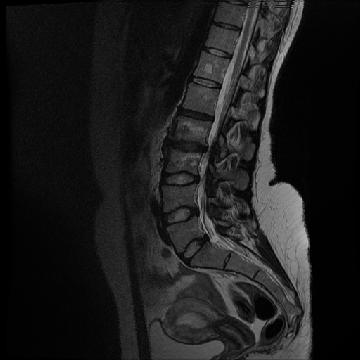
\includegraphics[width=.32\textwidth]{images/orig_usieg8_s22.jpg}
    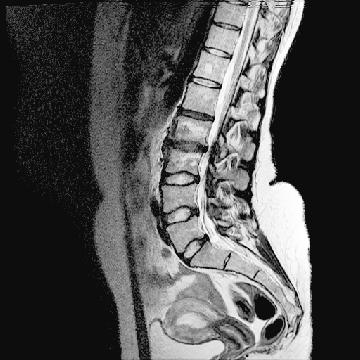
\includegraphics[width=.32\textwidth]{images/hist_usieg8_s22.jpg}
    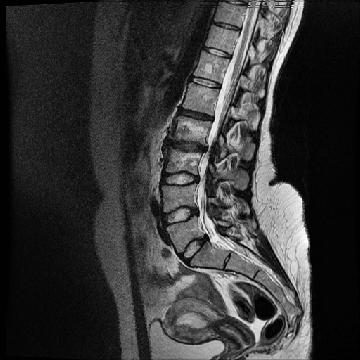
\includegraphics[width=.32\textwidth]{images/clahe_usieg8_s22.jpg}
    \caption{Image: 22$^{th}$ sagittal slice of the 8$^{th}$ image of the USiegen dataset. 
    From left to right, the original image, the image after ordinary histrogram contrast enhancement and the result after \acrshort{clahe}.
    The images show that \acrshort{clahe} avoids increasing the noise in the larger dark areas while resulting in a more balanced image than the ordinary histogram method.
    }
\end{SCfigure}

\acrfull{clahe} is an improvement on adaptive histogram equalization.
Limiting the contrast amplification avoids that noise is amplified in (near) constant regions of the image.
The parameters of this operation were adjusted manually.
Based on trial and error iterations, where the quality of the contrast improvement was estimated with the human eye based on visualizations from all datasets,
the following parameters were chosen:
\begin{description}
    \item[Number of grey bins:] 256 (maximum possible when working with 8-bit encoded images).
    \item[Kernel size:] 50. This parameter defines the extent of the \textit{local} region used by the algorithm.
    \item[clip limit:] $9.10^{-3}$. This parameter suppresses noise in the darkest regions (which contain the least information).
\end{description}

\section{Train, validation and test split considerations\label{sec:trainValTestSplit}}

To allow evaluation of the models produced, a test set is split from the development set.
The objective is to evaluate how well a model generalizes to new data\footnote{
    New data is to be interpreted here as a new sample from \textit{the same population} as the development sample.
    Unfortunately, I cannot claim that the different datasets I collected indeed form a perfect representation of the population of medical images of the lumbar spine.}. 
To provide an honest estimate of the out-of-sample performance, the test dataset should represent the investigated population and (hidden) correlations with elements of the development sample should be avoided.

This is done\footnote{
    To accomplish this, I used the function \texttt{GroupedStratifiedSplit} at \url{https://github.com/scikit-learn/scikit-learn/pull/18649/}. 
    This class is not yet part of the official \texttt{sci-kit learn} library release (at the time of writing) but functions well for this application.} taking into account the following:
\begin{description}
    \item[Stratified data:] The combination of data from different sources is stratified. Every source is considered a subpopulation. The data split is made such that the proportion of scans originating from each data source in every split is proportional to their occurrence in the total population.
    \item[Grouped data:] The scans of the same patient can be assumed to be correlated to each other. These scans should not be spread over different splits. The data is split at patient level.
\end{description}

For each datasource, the intended split is $\frac{4}{6}$ for train set, $\frac{1}{6}$ for cross validation set and $\frac{1}{6}$ for test set.
This distribution is not perfect but acceptable, as is indicated by the values in table \ref{tab:summary_split}.

\begin{SCtable}[\sidecaptionrelwidth][h]
 
    \begin{tabular}{lrrr}
\toprule
split &  test &  train &  xval \\
source       &       &        &       \\
\midrule
MyoSegmenTUM &     9 &     33 &     9 \\
PLoS         &     4 &     14 &     4 \\
USiegen      &     2 &     14 &     1 \\
xVertSeg     &     2 &     10 &     3 \\
\bottomrule
\end{tabular}

    \caption{Number of volumes by datasource and by split. The scan volumes are split such that scans of the same patient are in the same split set.\label{tab:summary_split}}
  
  \end{SCtable}

  \begin{SCtable}[\sidecaptionrelwidth][h]
 
    \begin{tabular}{ll|lll|l}
    \toprule
    split        &            & test & train & xval & total \\
    source       & dimension  &      &       &      &       \\ \midrule
    MyoSegmenTUM & Transverse & 1989 & 7293  & 1989 & 11271 \\
                 & Frontal    & 1989 & 7293  & 1989 & 11271 \\
                 & Sagittal   & 720  & 2650  & 725  & 4095  \\
    PLoS         & Transverse & 1528 & 5348  & 1528 & 8404  \\
    USiegen      & Transverse & 733  & 5063  & 501  & 6297  \\
                 & Frontal    & 681  & 4276  & 1080 & 6037  \\
                 & Sagittal   & 145  & 1089  & 180  & 1414  \\
    xVertSeg     & Transverse & 759  & 2652  & 785  & 4196  \\
                 & Frontal    & 812  & 4163  & 1290 & 6265  \\
                 & Sagittal   & 812  & 4163  & 1290 & 6265  \\ \midrule
    total        & Transvers  & 5009 & 20356 & 4803 & 30168 \\
                 & Frontal    & 3482 & 15732 & 4359 & 23573 \\
                 & Sagittal   & 1677 & 7902  & 2195 & 11774 \\ \bottomrule
    \end{tabular}
    \caption{Number of slices by datasource and by split.
    These values might seem high, yet, the reader should not forget these image slices are highly correlated. 
    There is very little additional independent information comparing one slice with a slice taken just 1mm further.
    On top of this, there are many slices which only contain the background class and do not provide much information for the model to train on the lumbar vertebrae classes. 
    \label{tab:summary_split_slices}}
  
  \end{SCtable}

The result of this operation is detailed in appendix \ref{sec:appendix_split} on page \pageref{sec:appendix_split}.

\section{Cropping\label{sec:cropping}}
The networks used require input images of size $352 p \times 352 p$, corresponding to $352 mm \times 352 mm$.
The image slices have different dimensions.
The incoming images are cropped or padded, depending on whether the image dimension is smaller or larger than the crop window.


When the image is cropped, one of 5 crops is selected, see figure \ref{fig:crop}:
\begin{description}
    \item[crop 0:] Crop from the top left corner of the image.
    \item[crop 1:] Crop from the top right corner of the image.
    \item[crop 2:] Crop from the bottom left corner of the image.
    \item[crop 3:] Crop from the bottom right corner of the image.
    \item[crop 4:] Center crop of the image.  
\end{description}

Not all slices are sufficiently large to produce 5 different crops. This is illustrated in figure \ref{fig:smallcrop}. In this case, one of the slice dimensions must be padded (symmetrically) to obtain an image of the desired dimensions.

When a slice is fetched from the train set, a random crop is selected from these 5.
This adds an extra level of variance to the training data. This avoids, for example, that the network learns that the spine is always at the same location in the images.

For the slices sourced from the cross-validation and train set, however, reproducibility is essential.
For each slice, the crop number is fixed.
This way, the cross-validation metric, evaluated to avoid overfitting is always calculated on the same images.

When reconstructing the volumes, in the second step of the model concept (see chapter \ref{sec:model_concept}), 
all different crops are evaluated in the model, and the responses for these crops are joined by averaging the model responses in the overlap regions.

\begin{SCfigure}[][htb]
    \centering
    \begin{minipage}{.99\textwidth}
        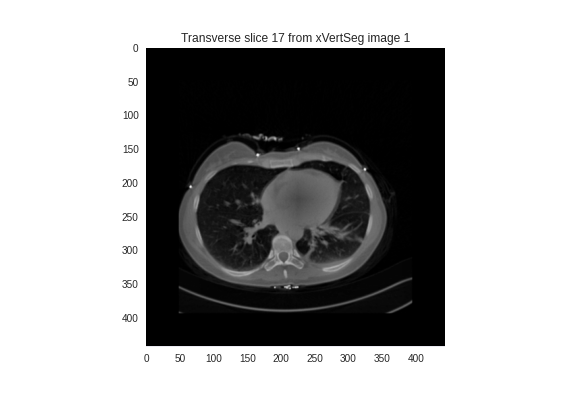
\includegraphics[width=.99\textwidth]{images/slice017.png}
    \end{minipage} 
    \begin{minipage}{0.99\textwidth}
        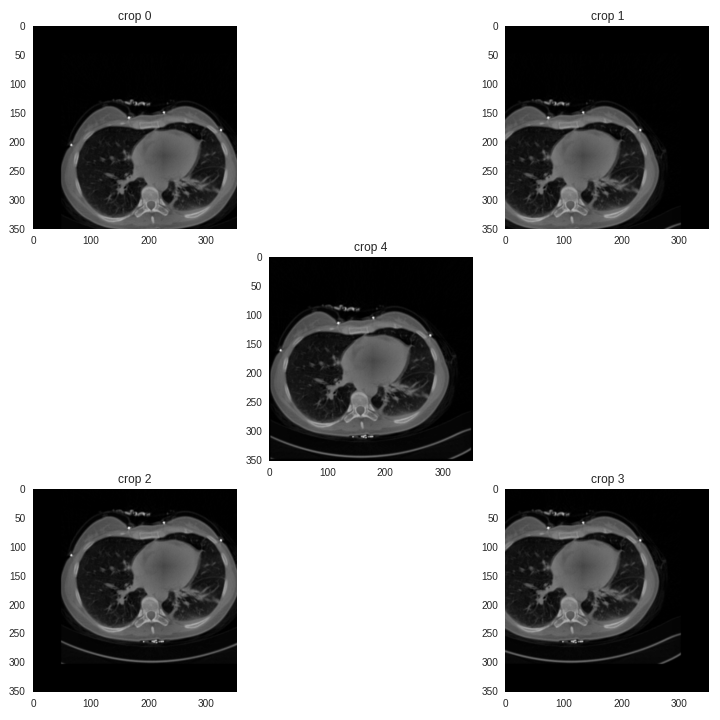
\includegraphics[width=.99\textwidth]{images/cropping_slice017.png}
    \end{minipage}
    \caption{
        Illustration of image cropping where the image is larger than the crop window dimensions. The original size of the image is $443 \times 443$, and the crop window used has dimensions $352 \times 352$.
        Crop 0 to 4 are 5 different images but have a considerable overlap. This means that in chapter \ref{sec:combination} on page \pageref{sec:combination}, 
        where the volumes are reconstructed from all relevant crops, for this type of slices four crops (0, 1, 2 \& 3) have to be calculated.\label{fig:crop}
        }
    
\end{SCfigure}

\begin{SCfigure}[][htb]
    \centering
    \begin{minipage}{.99\textwidth}
        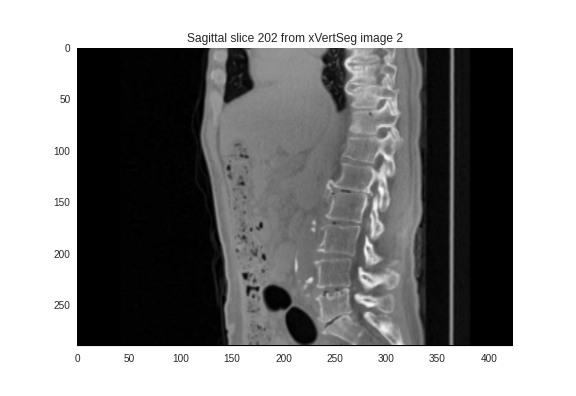
\includegraphics[width=.99\textwidth]{images/slice202.png}
    \end{minipage} 
    \begin{minipage}{0.99\textwidth}
        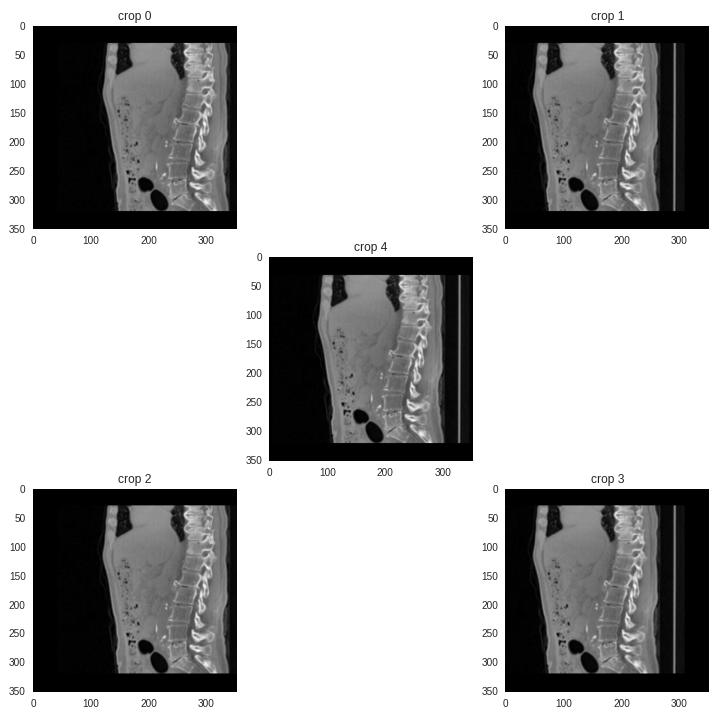
\includegraphics[width=.99\textwidth]{images/cropping_slice202.png}
    \end{minipage}
    \caption{
        Illustration of image cropping where the image is larger than the crop window dimensions.
        The original size of the image is $291 \times 424$, and the crop window used has dimensions $352 \times 352$.
        Crop 0 to 4 are not all different images. Since the image height is lower than the crop window height, this dimension is padded, not cropped.
        This results in crop 0 being equal to crop 2 and crop 1 being equal to crop 3. This means that in chapter \ref{sec:combination} on page \pageref{sec:combination}, 
        where the volumes are reconstructed from all relevant crops, for this type of slices only two crops (0 and 1) have to be calculated.
        \label{fig:smallcrop}
        }
    
\end{SCfigure}